\documentclass{article}

\usepackage{url}
\urldef\myurl\url{https://docs.microsoft.com/en-us/dotnet/framework/data/adonet/ef/security-considerations#:~:text=The%20Entity%20Framework%20does%20not%20enforce%20any%20security%20permissions%20and,store%20and%20by%20your%20application.}
\urldef\urlTit\url{https://scantitan.com}
\urldef\urlScanHost\url{https://hostedscan.com}

% Language setting
% Replace `english' with e.g. `spanish' to change the document language
\usepackage[english]{babel}
\usepackage{float}
\usepackage{tabularx}
\usepackage{parskip} 
\usepackage{mathtools}
% Set page size and margins
% Replace `letterpaper' with`a4paper' for UK/EU standard size
\usepackage[letterpaper,top=2cm,bottom=2cm,left=3cm,right=3cm,marginparwidth=1.75cm]{geometry}

% Useful packages
\usepackage{amsmath}
\usepackage{graphicx}
\usepackage[colorlinks=true, allcolors=blue]{hyperref}

\title{DevOps, Software Evolution and Software Maintenance}
\author{Alekxander Baxwill (abax@itu.dk)\\ \\ Jacob Sjöblom (jsjo@itu.dk) \\ \\ Frederik Peter Volkers (frvo@itu.dk) \\ \\ Albert Bethlowsky Rovsing (arov@itu.dk) \\ \\ Rasmus Andreas de Neergaard (rade@itu.dk)} 

\begin{document}
\maketitle

\begin{figure}[H]
\centering
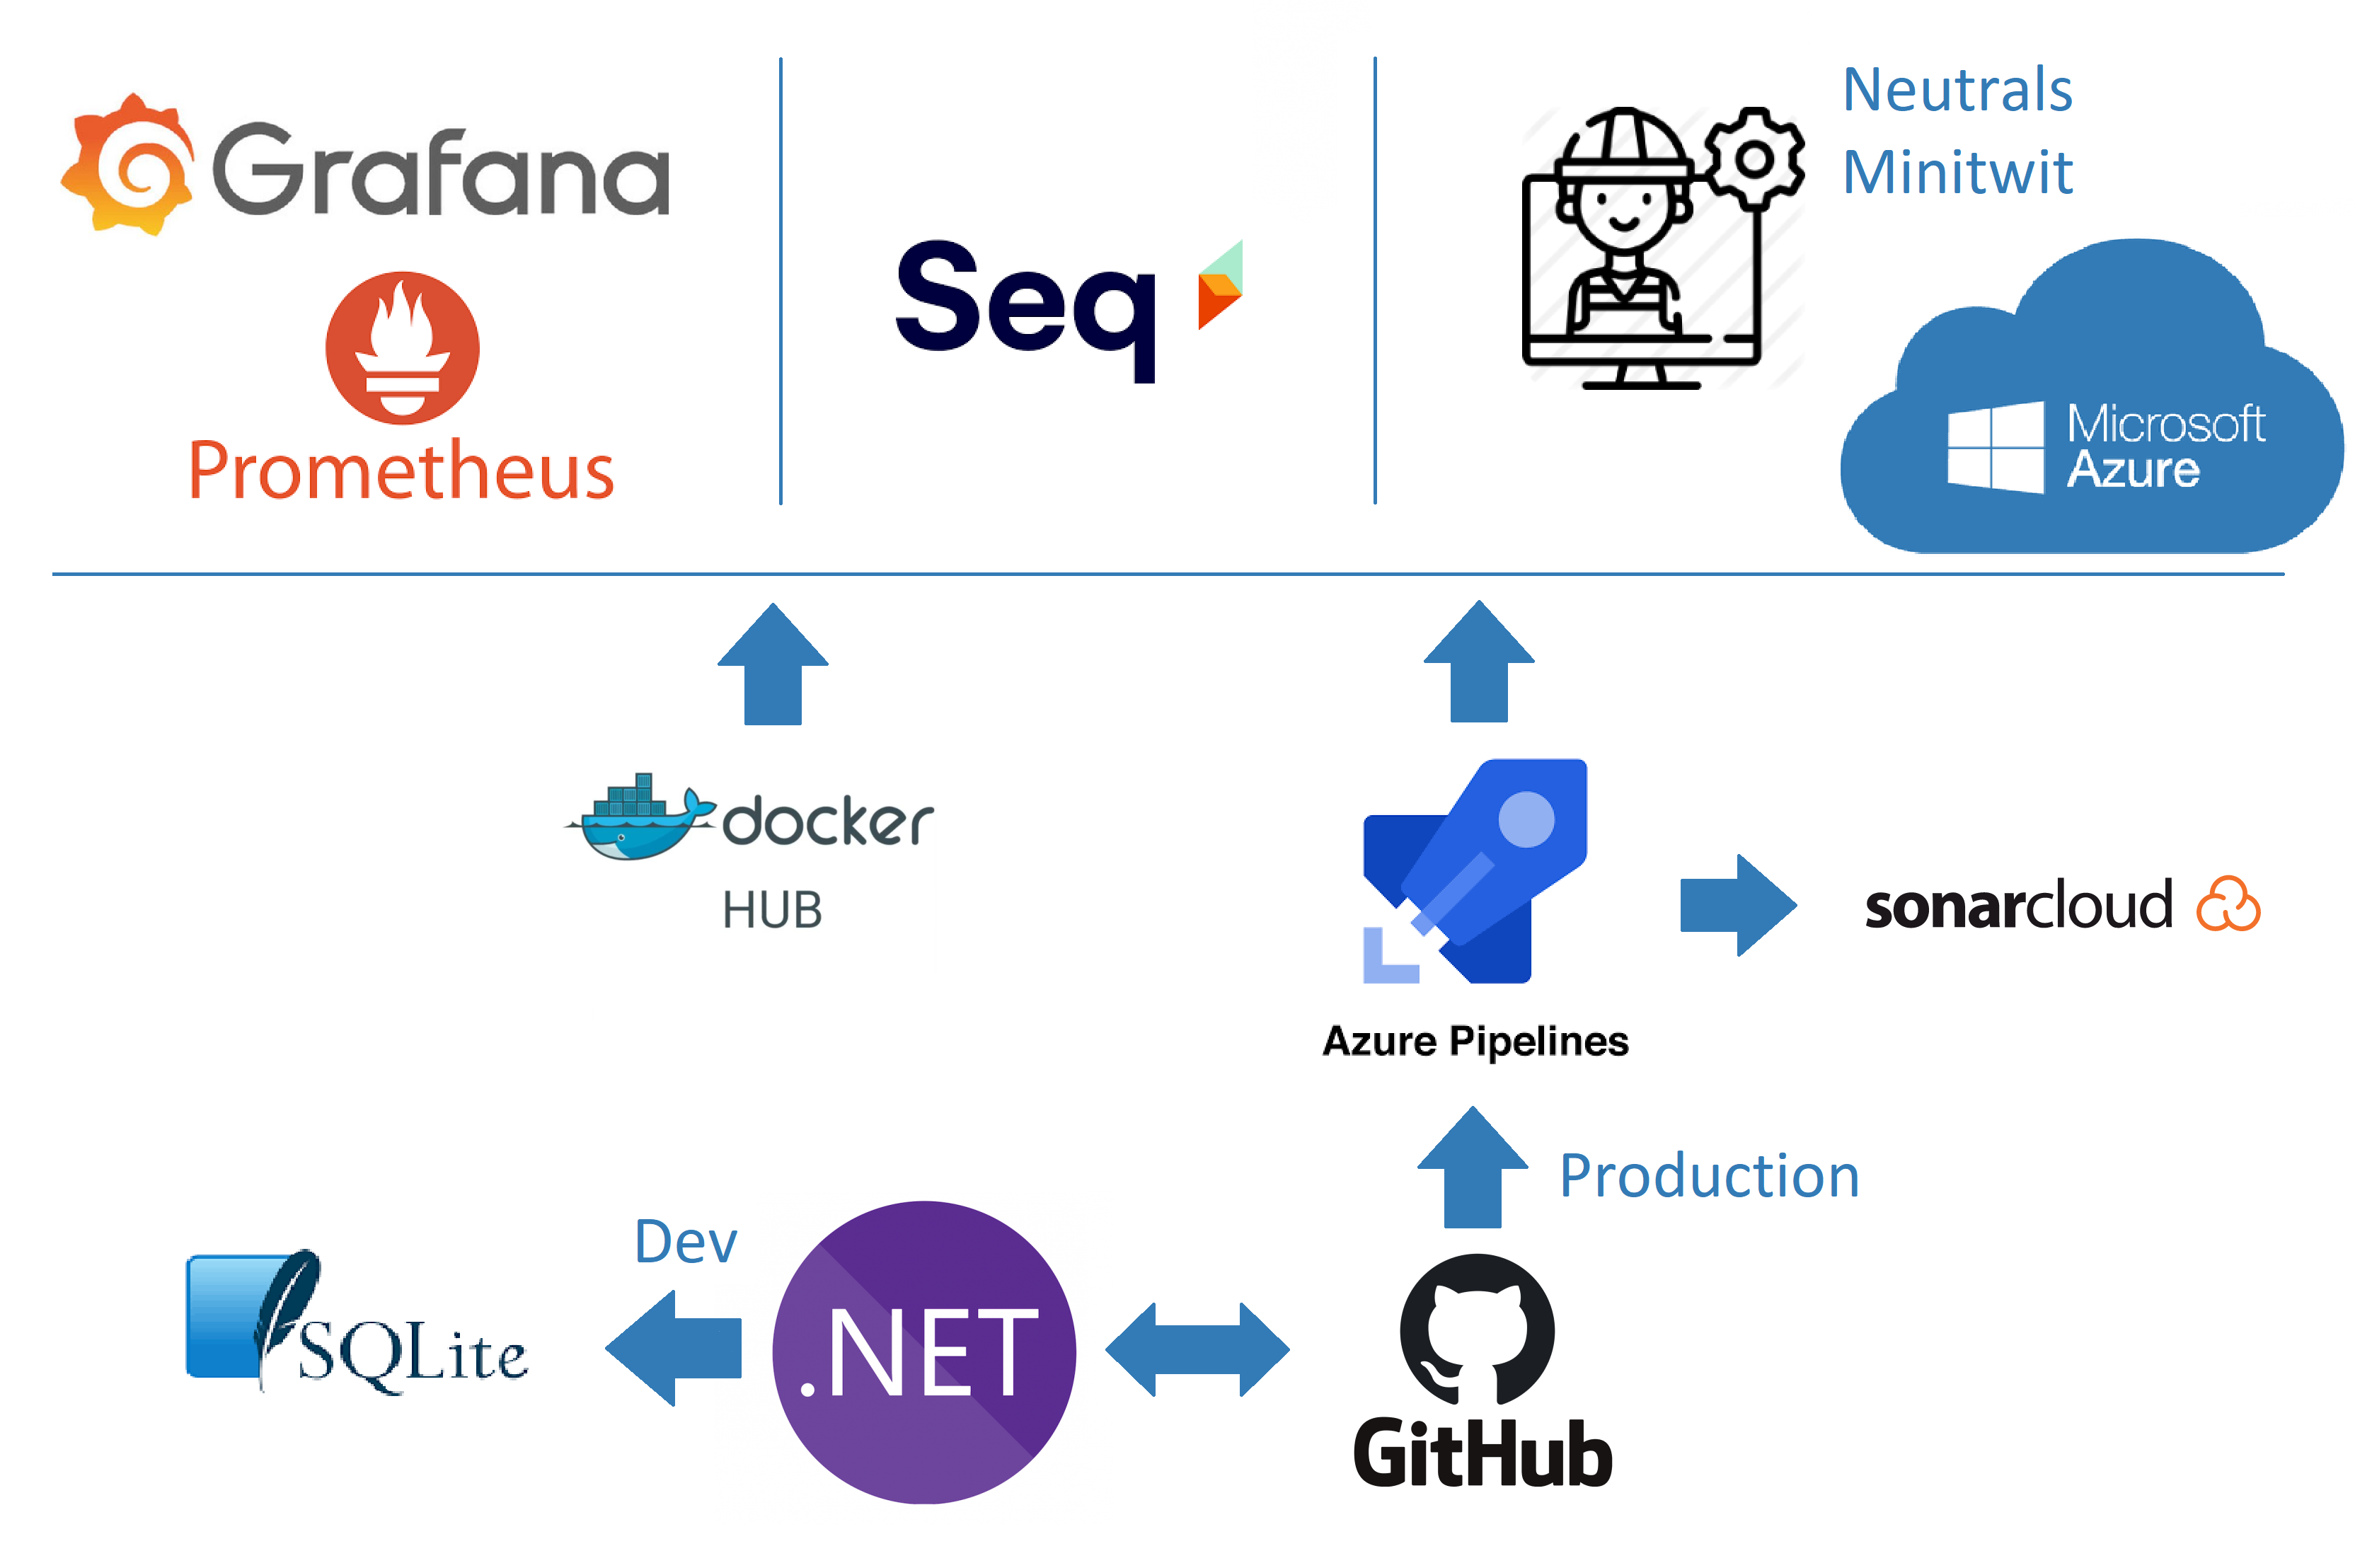
\includegraphics[width=1\textwidth]{images/SystemDesign.png}
\end{figure}

%Checklist/skeleton: https://github.com/itu-devops/lecture_notes/blob/master/REPORT.md
% revised idea for skeleton:
\newpage
\section{System's Perspective}
% skriv hvorfor vi vælgeer c# azure og asp.net
\subsection{Design and Architecture of the system}
As a basis for this project, we as a team decided on rebuilding the solution in the C# language. As a alternative Java was also discussed, since there was previous experience with it in the group. We decided on C# over Java to give our self an opportunity to explore a new language, while still having some experience to fall back on due to the similarities between the two. In addition C# is widely used in the industry, and gaining experience with .NET could be good addition to our future job aspects.

For the cloud provider, Digital Ocean was initially considered but due to the synergy between Microsoft Azure and other Microsoft Services (Azure DevOps, Azure SQL, Monitoring etc.) in addition to some team members having experience with Azure. Microsoft Azure also provides students with free credits.

To give an overview of the architecture and design of the MiniTwit application, the 3+1 approach is used.
The architecture of our MiniTwit implementation is based on a ASP-NET MVC which is based of the Model-View-Controller pattern. 



\begin{figure}[H]
\centering
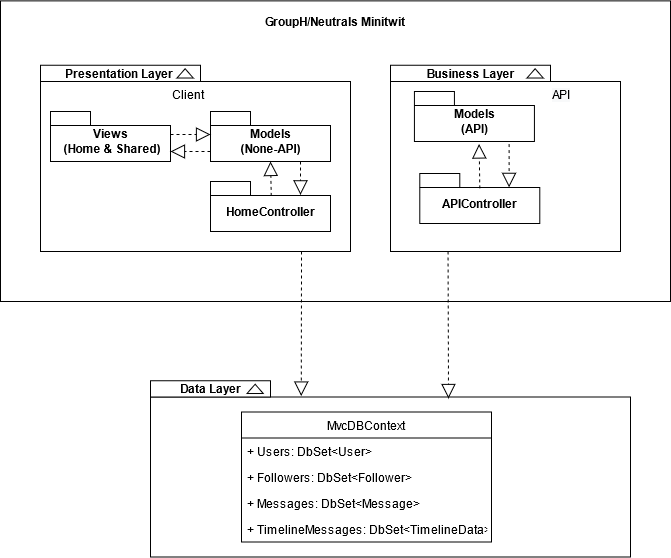
\includegraphics[width=1.1\textwidth]{images/Module View (3+1).png}
\caption{\label{fig:modview} Module View from 3+1}
\end{figure}

\begin{figure}[H]
\centering
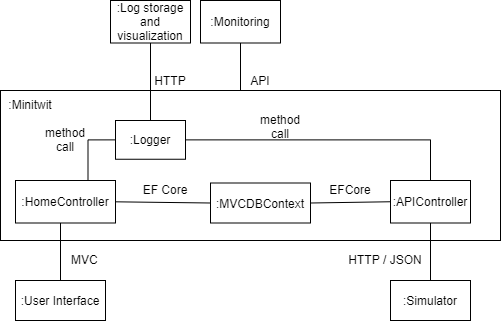
\includegraphics[width=1.1\textwidth]{images/Connector & Component View Point.png}
\caption{\label{fig:modview}Connector & Component View}
\end{figure}

\subsection{Dependencies}
\subsubsection{Software dependencies}

The dependencies of the system is derived via GitHub from the \texttt{mvc-minitwit.csproj} 
and \texttt{HomeControllerTests.csproj} project files. These correspond to the MiniTwit and testing project respectively. The dependency graph can be found on \url{https://github.com/albertbethlowsky/DevOpsGroupH/network/dependencies}. A small snippet of the current graph for both projects can be seen below:
\begin{figure}[H]
\centering
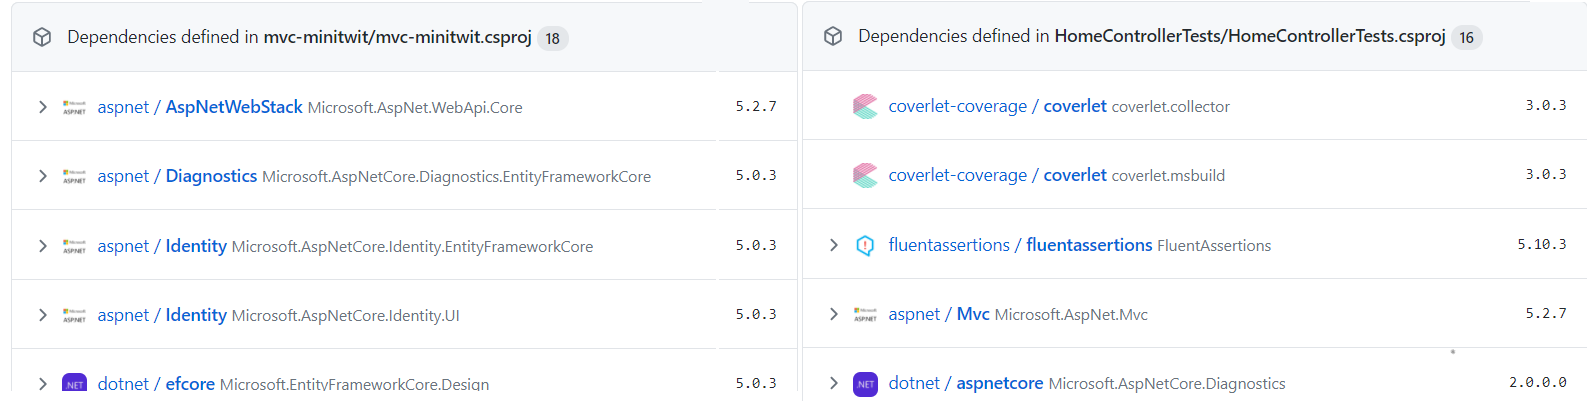
\includegraphics[width=1.1\textwidth]{images/dependencies-snip.png}
\caption{\label{fig:dep1}Snippet of dependency graphs from GitHub of both \texttt{mvc-minitwit.csproj} and \\\\ \texttt{HomeControllerTests.csproj}}
\end{figure}

With the use of NDepend we can provide a more detailed visualization, showing the concrete package dependencies. It is a static analysis tool which generate a dependency matrix for the backend dependencies. From the snippet of the matrix \ref{fig:matrix}, we can observe that the \emph{'mvc-minitwit'} package (row) is used by 20 code elements (blue) in \emph{'mvc-minitwit.Views'} (column) and \emph{'mvc-minitwit'} (column) is using 5 code elements (green) from \emph{'mvc-minitwit.Views'} (row) \cite{Ndepend}.
\begin{figure}[H]
\centering
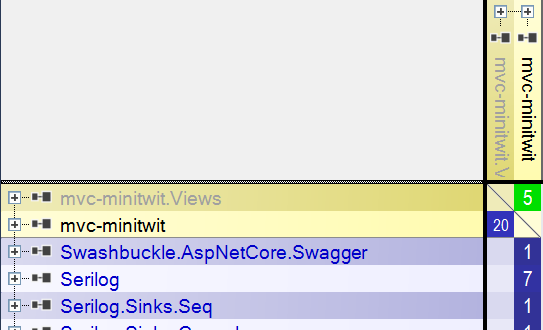
\includegraphics[width=0.7\textwidth]{images/ndepenmatrix.png}
\caption{\label{fig:matrix} Snippet of Ndepend - Dependency Matrix}
\end{figure}


\subsubsection{Cloud dependencies}
These dependencies are related to the services hosted on cloud-based domains.

\begin{table}[H]
\begin{tabularx}{\textwidth}{|l|l|l|X|}
\hline
    \textbf{Name} & \textbf{Service} & \textbf{Provider} & \textbf{Description} \\ \hline
    neutrals-minitwit & App Service & Microsoft Azure & development, rollout and scaling of web apps (.NET application) \\ \hline
    minitwit-neutrals & App Service & Microsoft Azure &development, rollout and scaling of web apps (prometheus, grafana) \\ \hline
    neutralsseq & App Service & Microsoft Azure & development, rollout and scaling of web apps (Datalust - Seq) \\ \hline
    minitwit-neutrals & SQL Server & Microsoft Azure & Hosting of SQL database \\ \hline
    minitwitDb & SQL database & Microsoft Azure & SQL database \\ \hline
    ASP-NeutralsRG & App Service Plan & Microsoft Azure & Hosting of Web Services (.NET application and Datalust - Seq) \\ \hline
    ASP-mvcminitwit & App Service Plan & Microsoft Azure & Hosting of Web Services (Grafana and Prometheus) \\ \hline
\end{tabularx}
\end{table}

%how does components talk together.. e.g. Sequence diagrams
\subsection{Current state of the system} 
With the help of different static analysis tools, it's possible to get a sense of the state of the system, including an estimation of the technical debt. Their respective results are briefly presented:

\subsubsection*{SonarCloud}
Based on the results from SonarCloud the systems seems to be in a satisfactory state, however there are a few caveats to point out. The auto-generated contents of \texttt{Migrations/}, and the \texttt{wwwroot/lib} folder has been excluded from all analysis since the latter contains deprecated jQuery libraries. These were given from the beginning, and were thus deemed out of scope to fix with time available. 

\begin{figure}[H]
\centering
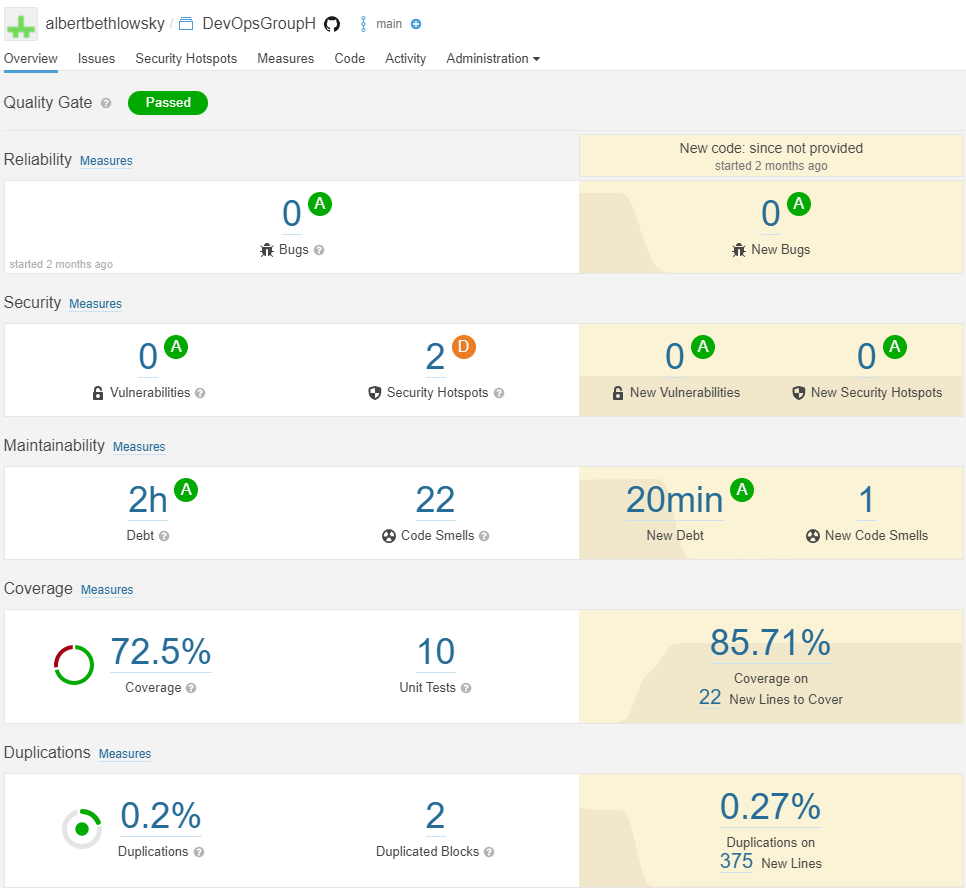
\includegraphics[width=0.7\textwidth]{images/sonarcloud.png}
\caption{\label{fig:dep1} Results from SonarCloud and its different categories, with the Quality Gate passed}
\end{figure}

The boiler plate, initialization files \texttt{Program.cs}, \texttt{Startup.cs} are excluded from test coverage analysis. \texttt{HomeController.cs} is also excluded from test coverage due to project scope and challenges with mocking cookies.
% her antages at læser ved hvad HomeController.cs er
From the maintainability category, there's "2 hours" of debt, but it's worth mentioning that it's a relative estimate based on "Code smells", uncovered and duplicated lines. This estimate should be compared with the estimates from the other tools.   
\subsubsection*{Code Climate}
The repository has a maintainability grade of "B", which with their estimates would be about 2 days of technical debt. There are 19 issues in total, split into 8 of duplication and 11 code smells. The file with the lowest maintainability score is \texttt{HomeController.cs} and has a "C", which would be the file to prioritize first for refactoring. The same files and folders have been excluded as with SonarCloud. %check this

As a side note a big source of the issues in both \texttt{HomeController.cs} and \texttt{APIController.cs} comes in the shape of \textit{"Avoid too many return statements"}. This is an issue that can be taken with a grain of salt, since it relates to the debate of "clean OOP" approach, which is harder to implement in server/API application. %let me know if u agree/disagree here  


\begin{figure}[H]
\centering
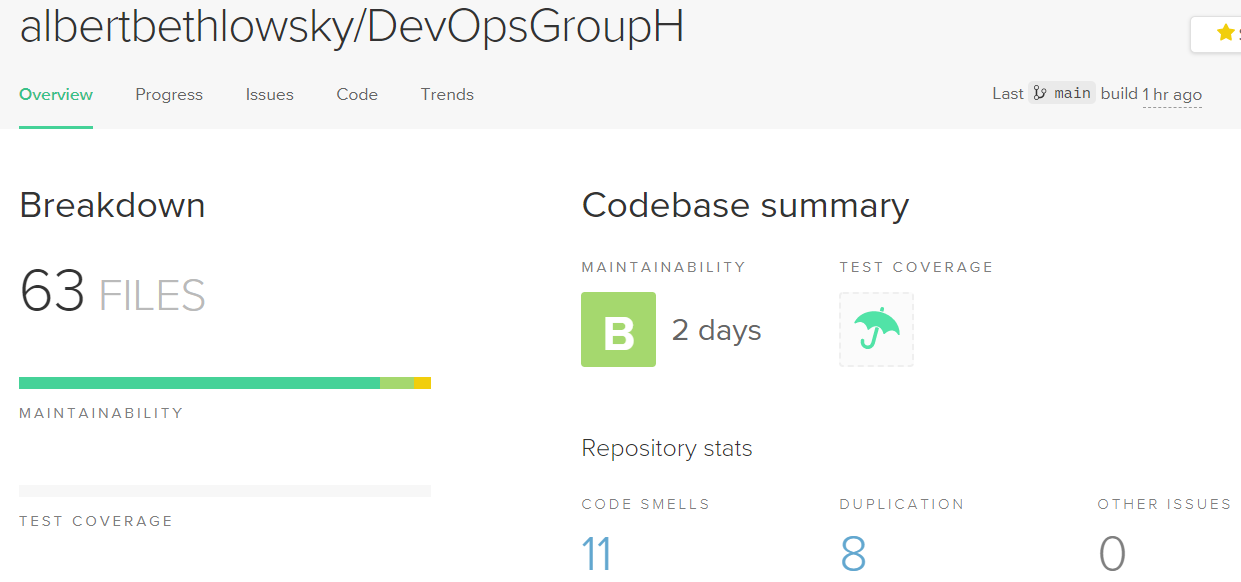
\includegraphics[width=0.7\textwidth]{images/codeclimate.png}
\caption{\label{fig:dep1} Code Climate summary and overview}
\end{figure}

\subsubsection*{Better Code Hub}
Better code hub rates our compliance 7/10 and gives us many of the same code smells as the other service scans have given us. We acknowledge that our lack of experience with C\# has some effects of on our coding style. 

\begin{figure}[H]
\centering
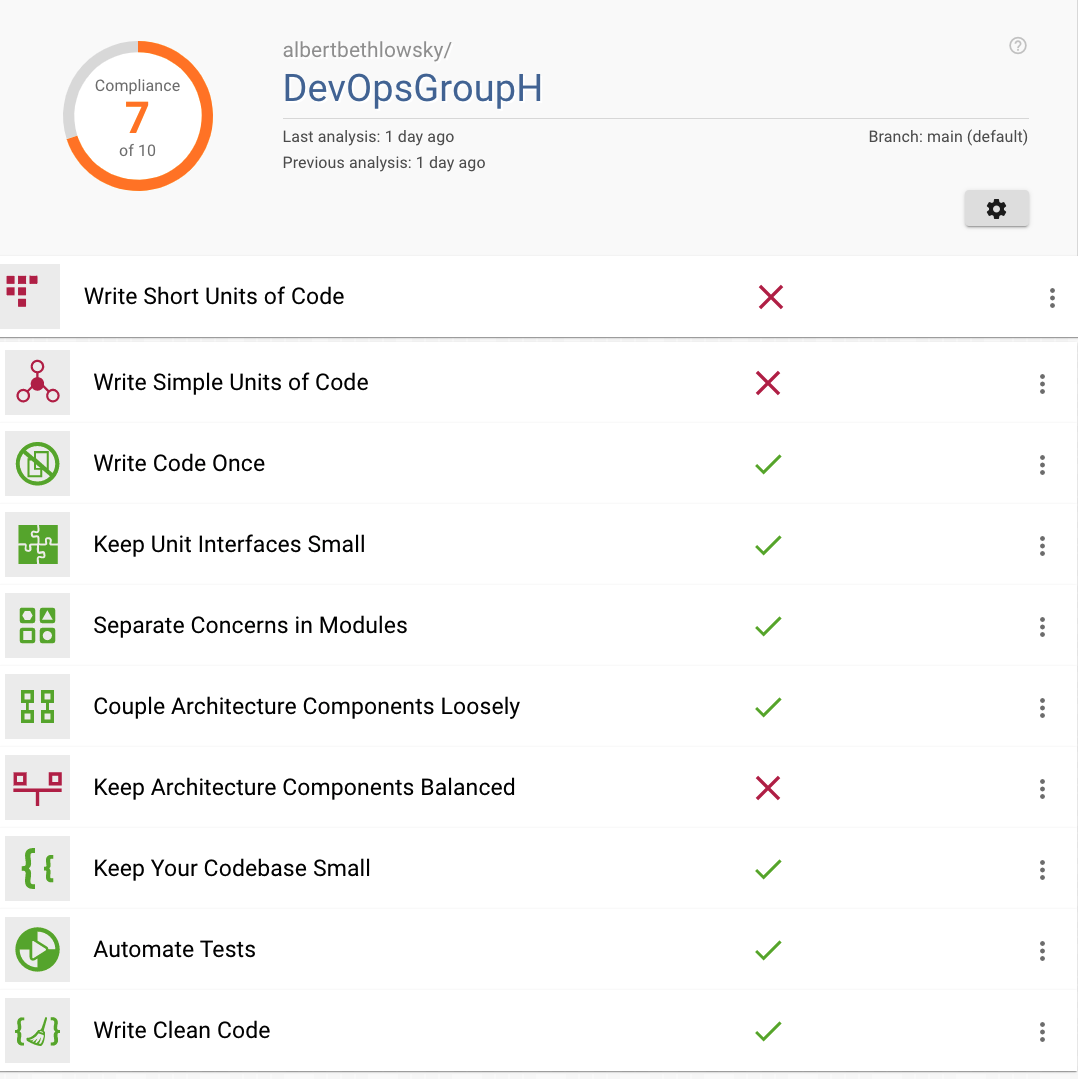
\includegraphics[width=0.7\textwidth]{images/bch.png}
\caption{\label{fig:dep1} Better Code Hub results}
\end{figure}

It's worth mentioning that technical debt is a relative term, and as seen between the tools, can vary quite a lot (e.g. 2 days to 2 hours).

\subsection{Licenses and compatibility}
The dependencies in our project are licensed under three licenses. The Apache 2.0 license \footnote{https://github.com/dotnet/aspnetcore/blob/main/LICENSE.txt}, the MIT license \footnote{https://opensource.org/licenses/MIT} and the BSD-3 clause \footnote{https://opensource.org/licenses/BSD-3-Clause}. All of these licenses fall within the category of permissive licenses. 
Below is a table showing how the dependencies are distributed on these different licenses. 
\begin{table}[H]
    \small
    \begin{tabular}{|l|l|l|l|}
        \hline
        Apache 2 License                            & MIT License                 & BSD 3      \\ \hline
       Aspnet/AspNetWebStack                  & Coverlet-coverage/coverlet    & Moq4/moq4      \\
       Aspnet/Diagnostics                     & Microsoft/vstest              &                \\
       Aspnet/hosting                         & Newtonsoft.Json               &                \\
       Aspnet/Identity                        & prometheus-net/prometheus-net &                \\
       Aspnet/Logging                         & Swashbuckle.AspNetCore        &                \\
       Aspnet/Mvc                             & Swashbuckle.AspNetCore        &                \\
       Dotnet/efcore                          &                               &                \\
       Donet/scaffolding                      &                               &                \\
       Serilog/serilog-aspnetcorer            &                               &                \\
       Serilog/serilog-filters-expressions    &                               &                \\
       Serilog/serilog-settings-configuration &                               &                \\
       Serilog/serilog-sinks-file             &                               &                \\
       Serilog/serilog-sinks-seq              &                               &                \\
       Fluentassertions/fluentassertions      &                               &                \\
       Xunit/xunit                            &                               &                \\
       Xunit/visualstudio.xunit               &                               &                \\
                                                                                                \hline
    \end{tabular}
\end{table}

As all licenses are permissive, they impose no restrictions for us as we do not modify the source code of the dependencies. As the majority of our dependencies are licensed under Apache 2.0, we have chosen to also license under Apache 2.0. 

\section{Process perspective}
\subsection{Interactions between developers and organization}
As everyone in the team have different schedules it was difficult to find time to always meet as a team. We strove towards having two weekly meetings on Mondays and Wednesdays. The meetings were held online on Teams, and in each meeting we presented what we were currently working on and what we had finished since last meeting. When we had to make big decisions we did it all together but when working on the project we often delegated the task between us. We assigned ourselves to tasks using Github Project Management. Often times team members would collaborate and do pair/group programming and work on tasks together. The communication of the team was exclusively through Teams to keep everything centralized.

\subsection{Description of CI/CD pipelines, stages and tools}
Azure DevOps is used to manage the CI/CD pipelines for the project. Azure DevOps was picked since it was easy to use and integrated well with the hosting on Azure. As an example, certain services (Azure Kubernetes Services, Azure App Service for deployment, etc.) for Azure could be used from the market place on Azure DevOps. %A feature that was helpful was the ability to insert yaml-templates for the services directly.  

There are two pipelines, the CI pipeline used for testing, code analysis and building and the CD pipeline for deploying. 

\subsubsection*{Continuous Integration}
Whenever the main branch is receives commits, the CI pipeline is triggered. The chain consists of one stage with the jobs executed in the order of: 
\begin{enumerate}
    \item Test and Sonar Cloud Setup and Analysis
    \item Build Image and Upload to Azure Container Registry 
    \item Make auto GitHub release (if tag added in commit)
\end{enumerate}

If testing fails the pipeline stops. The result of running the CI pipeline looks as follows:

\begin{figure}[H]
\centering
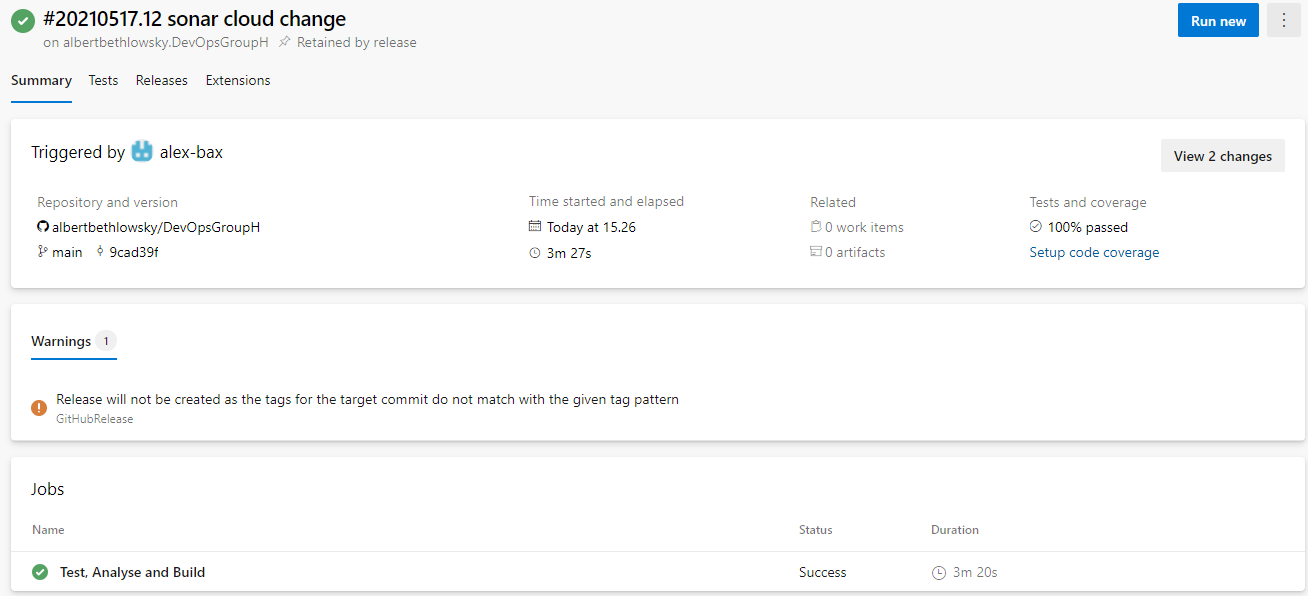
\includegraphics[width=1\textwidth]{images/pipeline-result.png}
\caption{\label{fig:res} Result of the CI chain from \texttt{azure-pipelines.yaml}}
\end{figure}

No automatic git branch-merging tasks have been added, which is reflected on in Lessons Learned section. % we should have had Pipeline setup on Dev such that we don't flood main with tiny releases + be sure that dev more frequently is acceptable state + be able to check much faster if your commit is acceptable 

\subsubsection*{Continuous Delivery}
The CD pipeline is responsible for pulling the latest image on ACR, and is thus triggered when a new image is pushed. ACR was chosen as the container registry for the MiniTwit image since it integrates more easily with Azure Kubernetes Services and Azure. After having pulled, a post deployment gate is checked, in this CD chain the status of a SonarCloud Quality Gate. Based on the results of the SonarCloud analysis from the CI pipeline the gate is updated, and if it passes the image is deployed onto Azure. Otherwise the release will timeout after 5 minutes and fail.   

\begin{figure}[H]
\centering
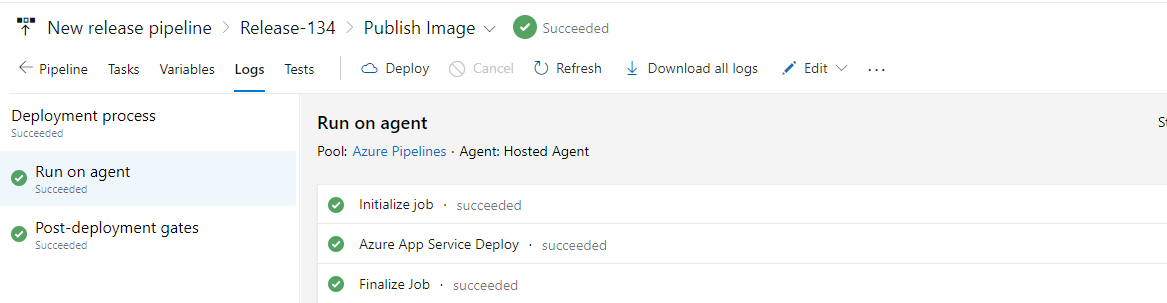
\includegraphics[width=1\textwidth]{images/devops-result.png}
\caption{\label{fig:release} CD pipeline}
\end{figure}


\begin{figure}[H]
\centering
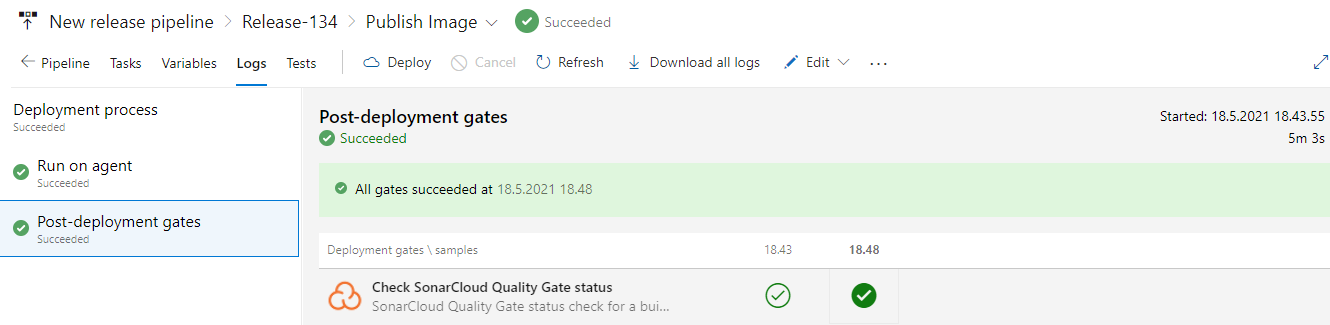
\includegraphics[width=1\textwidth]{images/post-gate.png}
\caption{\label{fig:gate} Passing SonarCloud Quality gate on the CD pipeline}
\end{figure}

% whenever a new a image is received on ACR, start Release pipeline
See \texttt{azure-pipelines.yml} for more details on the stages and tools used in the CI pipeline. Terraform will be applied to the pipeline in future iterations such that it will deploy all the services to Azure. %we ha automated the infrastructure (IaC) maintenance.  

\subsection{Repository arrangement/organization}
\subsection{Applied Branching Strategy}
Throughout the project a "Long-Running Branches" strategy has been used. The \textit{master} branch has primarily been used for code releases as pull requests from \textit{development} or \texttt{.yml} pipeline changes. The \textit{development} branch was used to merge all the feature branches back into, so that it in turn becomes can be merged into \textit{master} as the next stable release. 

Finally the individual feature branches correspond to the issues on the task board on GitHub. Each feature branch is named after their issue number, e.g. \texttt{fea#34APIController}. Feature branches are short lived, and are closed when done. 

Pull requests where inspected as a team or by another developer.
Automatic releases can be triggered by the CI pipeline, by adding a specific tag to a commit when merging into \textit{master}. Releases were however often done manually, since that way we could a provide a description/documentation to it. This had its drawbacks, one being that's it's somewhat against the DevOps idea, but also that we didn't release as often as we would have liked.   

\subsection{Applied development process and related tools}
\subsubsection*{Distributed workflow}
A "Centralized Workflow" was used, meaning that there's one shared repository, that every developer can collaborate on. This seemed fitting for the size of the code base and team.

\subsubsection*{Simple Kanban board}
We used Github's Projects for task identification, specification, and planning. The board consists of the traditional Kanban setup with 'tasks', 'in progress', 'parked', and 'done' as seen the fig \ref{fig:kanban}. Each week we would receive a list of tasks as an assignment for the course. Firstly, we listed them all within the 'tasks' lane. Secondly, we converted the tasks into issues and assigned group members to them. Thirdly, the tasks would be inserted into its retrospective lane. Then each Sunday we would gather up on the tasks completed on the assignment and review the code before a merge to the main branch was completed. 
\begin{figure}[H]
\centering
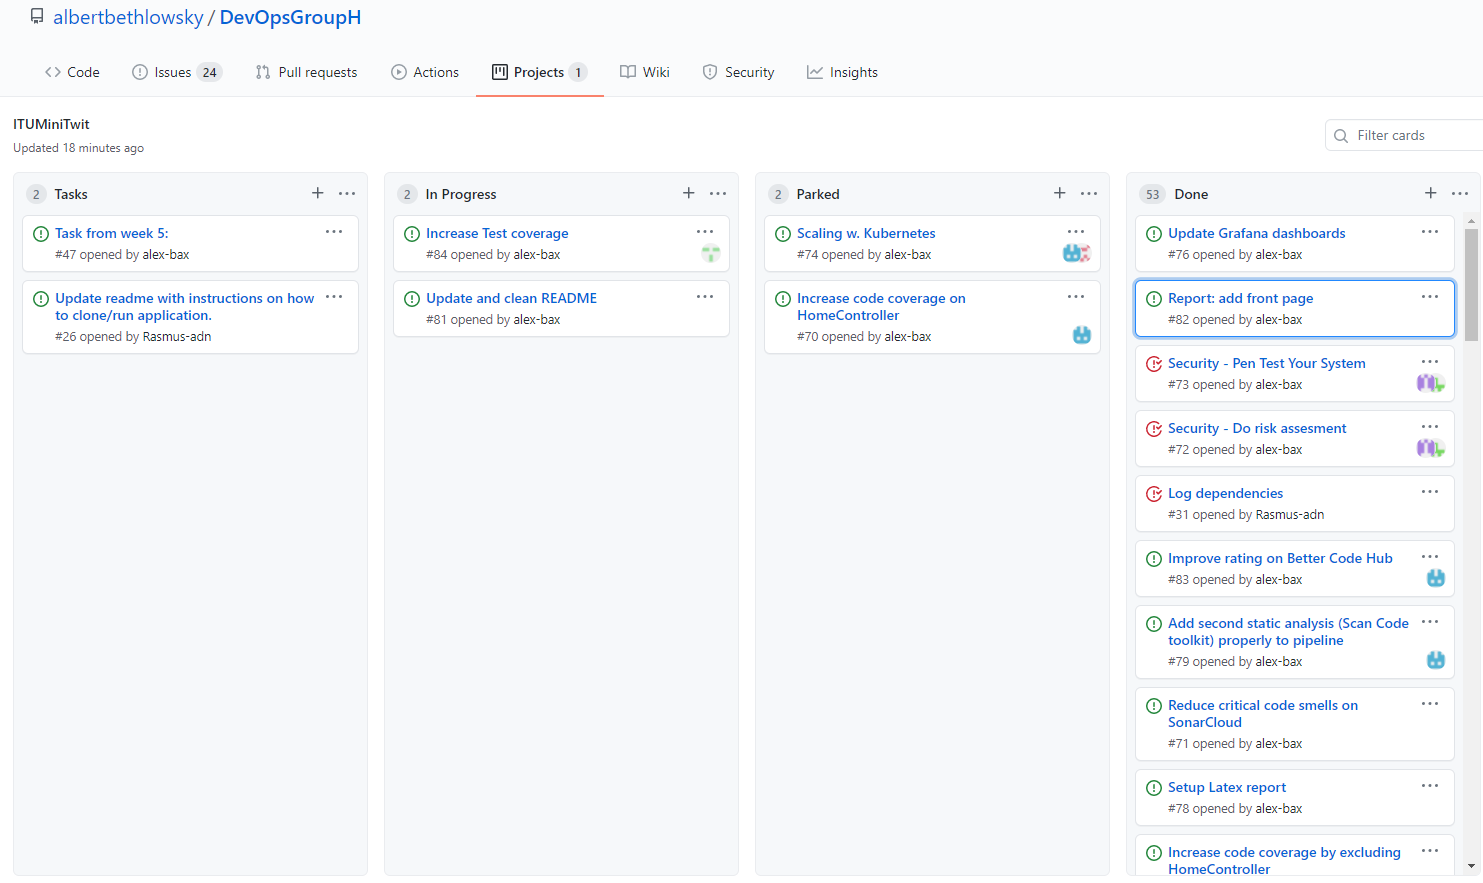
\includegraphics[width=1\textwidth]{images/kanban.png}
\caption{\label{fig:kanban} Github Project - Kanban Board}
\end{figure}
We decided to use Github Projects since we wanted to centralize as much of our work to one medium. Other mediums were also possible to use such as a simple excel sheet with a product backlog. Or online solutions such as monday.com, jira.com, or temgantt.com. However, we were concerned that utilizing an external solution from Github would result in less task management.  

\subsection{Monitoring}
% what are we logging 
For monitoring Prometheus was chosen to scrape the data from the MiniTwit container, and Grafana to visualize it. More precisely Grafana pulls data from the Prometheus container regularly, which in turn pulls data from the application through the /metrics access point of the website. The Prometheus and Grafana are deployed on containers on their own App Service, separate from the App Service hosting MiniTwit.

From quick research, these tools were chosen since they have good compatibility and documentation, but other alternatives to Prometheus such as DataDog could have been chosen as well.

To supplement Grafana, for example to get insights on metrics such as RAM usage, in and out-going data bandwidth usage, thread count, etc. we used the monitoring tools available on Azure for the services hosting MiniTwit and the SQL db. These stats are especially useful to determine the general load and whether or not to scale the server to meet demand.  
\begin{figure}[H]
\centering
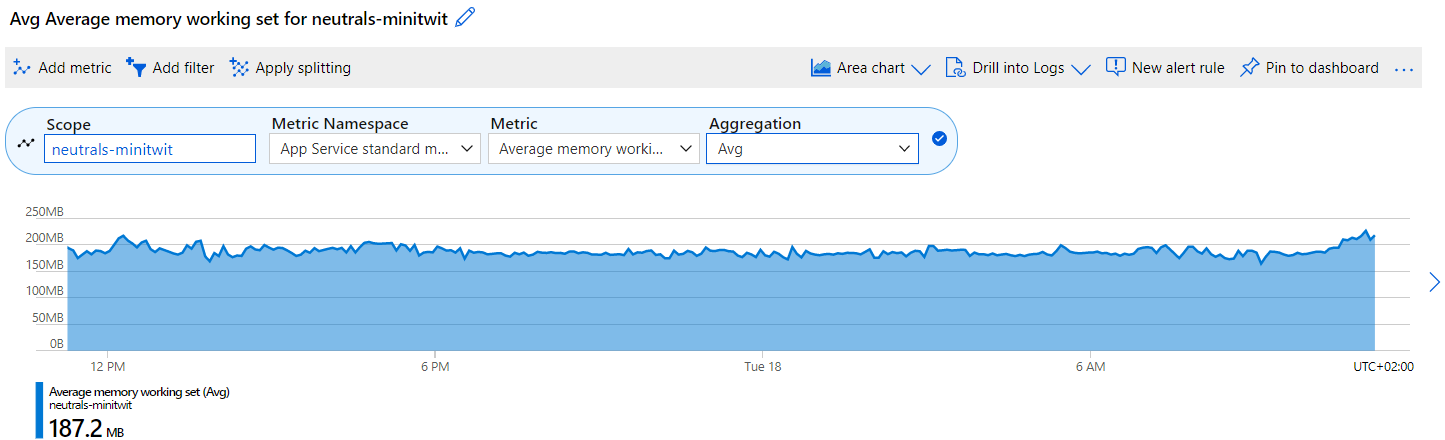
\includegraphics[width=1\textwidth]{images/azure-mem-usage.png}
\caption{\label{fig:RAM} Memory usage of MiniTwit container from the Azure App Service}
\end{figure}

\subsubsection{Dashboards on Grafana}
On Grafana the \textit{Rate of http calls} dashboard shows the number of different types of HTTP responses emitted from traffic on the endpoints over time. 

For example, from inspecting figure 10: at 18.00 there was about 2.5 thousand 204 status codes sent from the server on the endpoint of the form \texttt{https://neutrals-minitwit.azurewebsites.net/msgs/Joe}
triggering method \texttt{CreateMessageByUser()} in the API.     

This includes the most common HTTP status codes 2xx, 3xx, 4xx and 5xx. It gives a general overview of how the server responds to the traffic, and has been useful to indicate error trends.

Other dashboards used are: \textit{The duration of HTTP requests}, \textit{Total no. threads} and \textit{Request currently in progress}. 

% how are they deployed? both images on the same service (from docker compose)?

\begin{figure}[H]
\centering
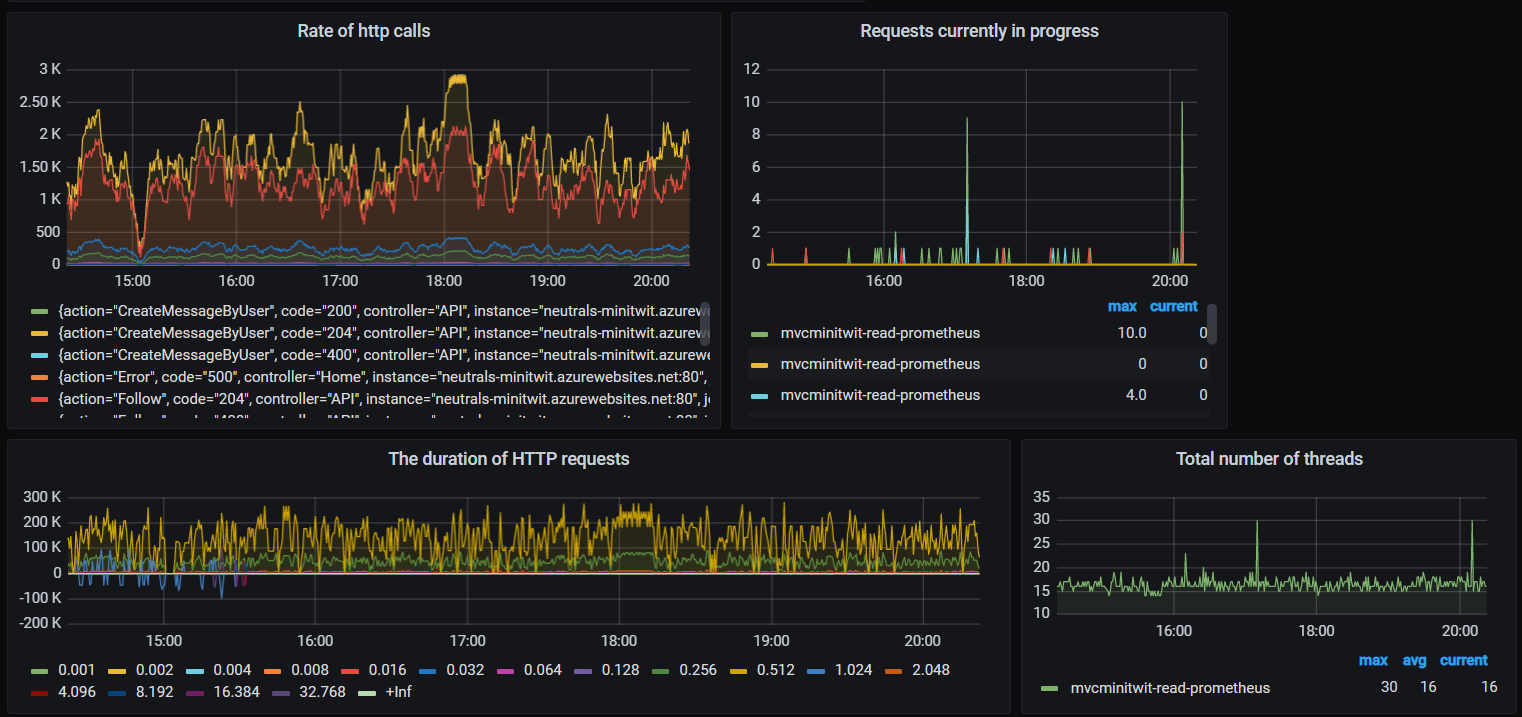
\includegraphics[width=1\textwidth]{images/dashboard.png}
\caption{\label{fig:dashboard} Grafana dashboards}
\end{figure}

In future iterations alerts from either Azure or Grafana could be considered. Also more in depth db monitoring could be implemented, since it was only shortly experimented with, tracking no. users and no. messages.

\subsection{Logging and log aggregation}
For purposes of logging, multiple different solutions were initially discussed within the group. The ELK stack introduced to us during the course, even though being very advanced, seemed difficult to implement into our system in comparison to its benefits. 
As an alternative we investigated the possibility of using Promtail together with Loki. These softwares offers the possibilities of applying the same methodology as Prometheus, but in contrast captures logging information, diverting it to Loki which in turn can aggregate the log information into Grafana.
This strategy proved more difficult than we expected, since working with Azure as our host displayed a lot of issues with opening and forwarding ports required to utilize these programs.
The experimentation with these solutions however did lead us to the use of Serilog, which ended up being our chosen solution for logging.
Serilog is injected on top of .NET's native logging infrastructure and provides easy enhancements to the log context in addition to log custom data points captured or generated within the system.
Serilog uses a sink to continuously send log data to Datalust Seq, which is the aggreation and visualization tool we opted to use.
Seq enables us to monitor multiple levels of the logged information within various timeframes that can be specified by the user.
In addition to this, the "Events" tab allows us to search and filter on all the aggregated logs, providing a simple approach to identifying overall trends and specific errors which might have occurred in the system.

Working with the MVC framework, the logging we perform are primarily centered around the controller section of the framework. All calls passing through the controller is logged with elevation "Information" or higher giving information in regards to call initiation and completion. In addition to this user defined log entries are created to provide additional information within each call for better errorhandling.

\begin{figure}[H]
\centering
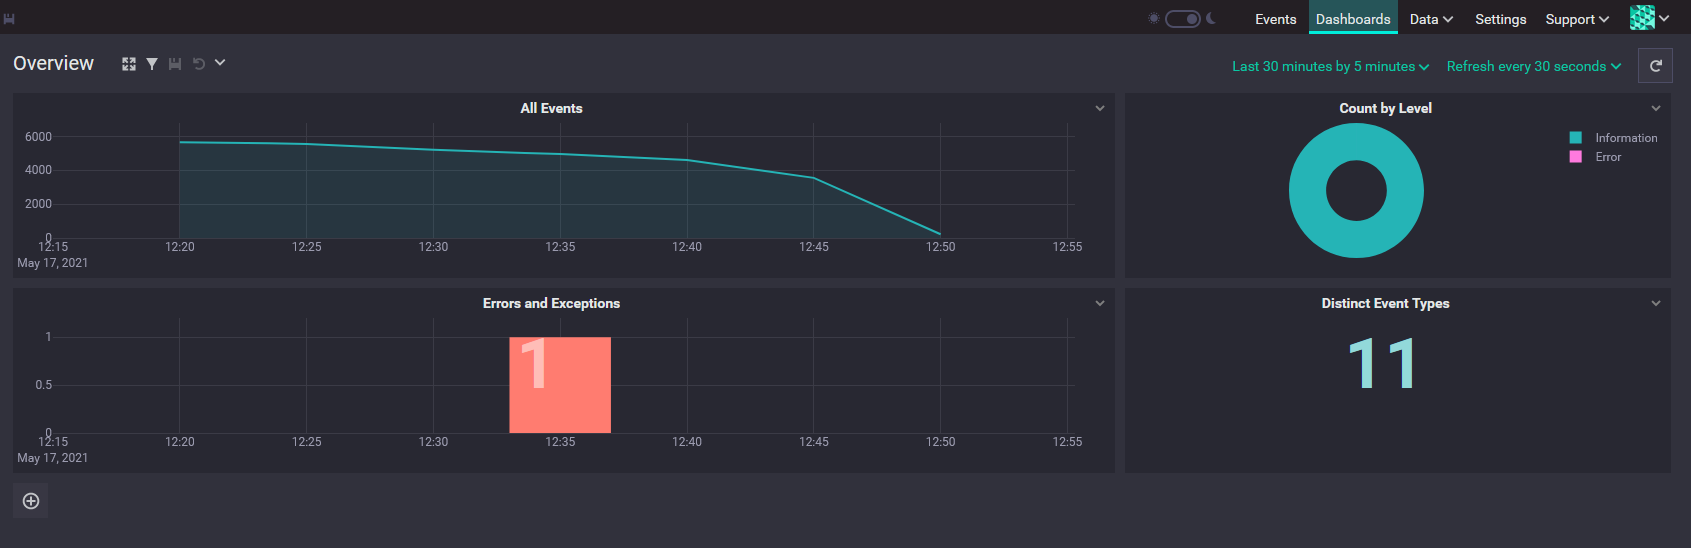
\includegraphics[width=1\textwidth]{images/DatalustSeq2.PNG}
\caption{\label{fig:seqdashboard} Datalust Seq dashboard}
\end{figure}

\begin{figure}[H]
\centering
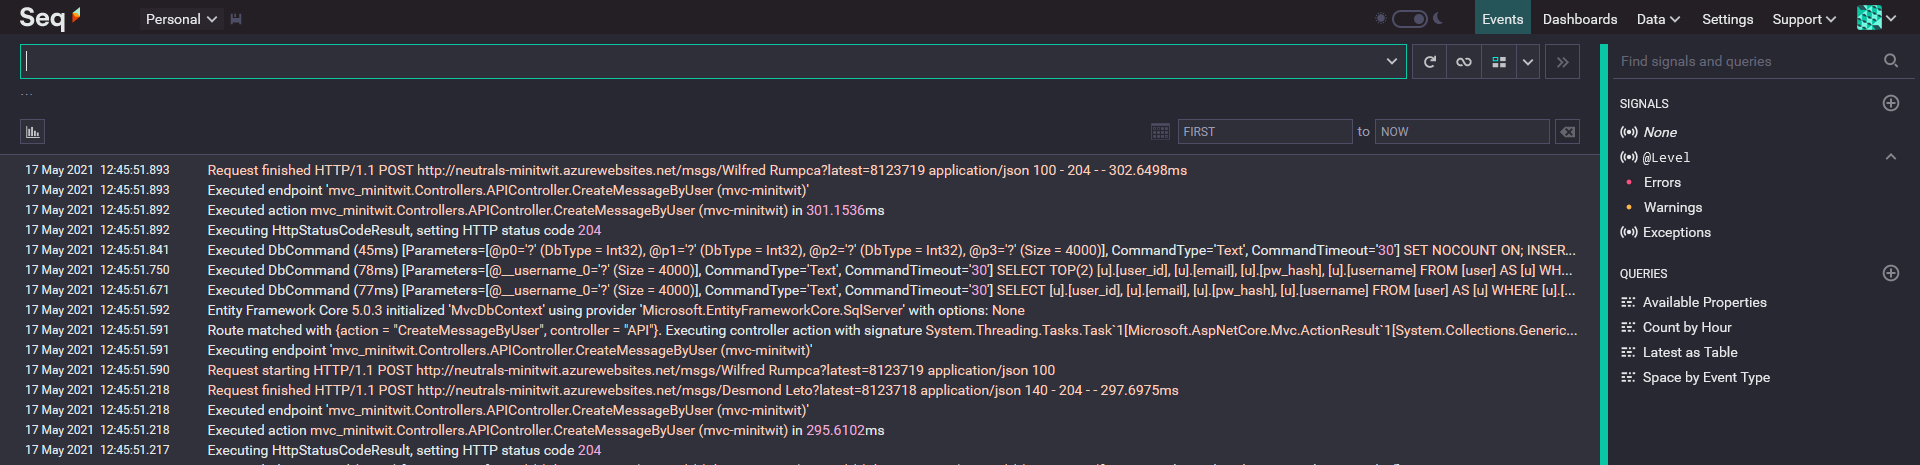
\includegraphics[width=1\textwidth]{images/DatalustSeq.PNG}
\caption{\label{fig:seqlog} Datalust Seq log}
\end{figure}

\subsection{Brief security assessment} 
While dotnet provides useful classes and services to write more secure code, a known security issue in our code is that we use 'Message-Digest algorithm 5' (MD5) for hashing the users' passwords. We are aware that MD5 is no longer considered secure as it has been cryptographically broken. Therefore using an alternative such as bcrypt or Argon2 would be a better alternative. The most secure hashing algorithm for passwords that is currently natively supported in dotnet is PBKDF2. Therefore we would have to be cautious if we were to use bcrypt or Argon2 as anyone can author a NuGet package. We consider this risk to be high. A way of overcoming the problem of the users having a password stored with the old hashing algorithm, we would have to make a check when the user logs in and then rehash their password with the new algorithm.

Furthermore we use versions of the JavaScript Libraries, jquery and bootstrap, that have known security vulnerabilities. To eliminate any risks we would have to upgrade the libraries to the newest version available. We consider this risk to be low. 
While we use use LINQ for our queries with our Entity Framework the system is not vulnerable to SQL injection.\footnote{\myurl} The Entity Framework provides standards that has generally helped us eliminate different vulnerabilities. We have prevented XSS, X-frame options and sniffing by setting security headers with the Use method directly in our Configure method in the StartUp.cs file. We have used ScanTitan\footnote{\urlTit} and Hostedscan\footnote{\urlScanHost} to pen test our system. 


\subsection{Applied scaling and load balancing strategy} 
We implemented azure's 'scale out' service which is a built-in feature that helps applications perform their best when demand changes. It enables our services to run on multiple Virtual Machines (three in our case) simultaneously and where the load will be balanced automatically. We applied this scale-out to multiple services running; Web App Services and Service Plans \cite{scaleout}. 
\\
\\
Moreover, we did try to establish Kubernetes services and incorporate it into our pipeline. However, we met multiple errors, both pricing tiers with azure and also authentication problems with the active directory. Simply put, ITU's active directory did not allow us to administrate Kubernetes on Azure. We also investigated the possibility of using docker swarm, but they are in a vanilla stage with azure and hence major errors occured when trying to implement. For example, this docker swarm template for azure is being linked by Microsoft and it fails almost all of their tests \cite{dockerswarm}.   


\section{Lessons learned perspective}
Throughout the lifetime of the project, numerous decisions have been made in good faith when considering the understanding of the overall project and it's technologies at those points in time. However as the project evolved from birth to it's current state, some of these prior decisions, showed to pose bigger obstacles for the project than anticipated at the time, as we will discuss in the following sections.
% moving db to Azure SQL - upgrade db with more DTU - 
% multiple fixes on API (adjustments in HTTP Status codes)
% should have considered indexing for the DB
\subsection{Evolution and refactoring} 
    \subsubsection{Language and Framework}
    Early on in the process, we quickly identified that going with .NET held major advantages in their offering of templates and wast majority of guidance online on multiple topics. The benefit of having information readily available when needing assistance, however also proved to serve as a disadvantage at certain times. The .NET framework spans across multiple iterations and versions  like .NETCore, .NETFramework, ASP.NET among others. Though NuGet packages are obtainable for most of the different versions, solutions to various problems were not always applicable to our approach and desired outcome. This of course was not expected at any given time, but with ongoing research and due diligence we improved at identifying which resources were relevant and which were outdated. This experience helped clearly showcase that during a refactoring process of a "legacy" software, choice of language is only one part of rebuilding the software into a more modern solution.

    \subsubsection{Database Management}
    Though a shift from SQLite into another DBMS was clear from the start, it became clear though, not having this transition in place in a timely manner can cause great complications as we had to experience the hard way.
    During the early stages of the simulator things looked to be running as intended, we however quickly after that, realized this was unfortunately not the case. We identified an issue with the API not posting certain messages and successfully following and unfollowing other users. Upon fixing the issue it occurred to us, we had mistakenly locked the database into the container image, thereby not being able to access any of the data stored from outside the system. After countless of hours spent trying to mitigate this error, we had to admit defeat and perform our migration into another DBMS with backup data from another group. This allowed us to carry through with the necessary fixes for the API and move on with the project. It was blatantly clear after this incident that decoupling of the software and the database is a high priority, or as a minimum ensuring proper access to it's content before going live. Since we are simulating a real life environment, this action resulted in the deletion of all users and messages which is far from ideal, since a backup from a third party under normal circumstances is highly unrealistic.

\subsection{Operation}
    \subsubsection{Foreshadowing}
    We define operations as the completion of the weekly assignments. Many struggles occurred at almost each weekly assignment due to steep learning curve. Many of us have not used many of the technologies suggested and therefore many obstacles had to be conquered.
    In addition to lacking required knowledge of the technologies we needed to implement, not taking into consideration the implementations of future features, occasionally lead to discrepancies in our system. Initially certain functionality was implemented on standalone basis, which worked for certain aspects of the system, but in time we got better at foreshadowing, basing technology and implementation decisions not only on our current tasks, but also tasks to come. Working agile holds huge advantages to being flexible during development, but without proper organization of items can also lead to mismanagement of time and resources. Overall having a filled out Kanban board or similar, with all development items to come, could have helped in guiding our decision making in the early stages of the project.

    \subsubsection{Azure}
    Azure as a service provider comes with countless baked in solutions supporting deployment, monitoring, health checks, logging and more, providing easy setup and maintenance of simple solutions. In regards to customization of our deployment however, Azure did prove to be very difficult to work with. Azure is comprised of many tiers of pricing, granting access to various possibilities within their services. Being on a budget and on an "Azure for Students" license, made of some of the weekly requirements for the course, very difficult to complete.
    One of the most noticeable obstacles worth to mention is the inability to access certain ports.
    Azure as a default provides www.{xxx}.azurewebsites.net as access points, not enabling port specification when accessing the website. This caused a lot of issues in instances where multiple technologies needed to be embedded into a docker compose file. Ultimately in rendered us unable to run our program together with Prometheus and Grafana as an example.
    With some tinkering we did discover the possibility of layering images on top of each other in situations where only one image needed to be displayed for usage. In the example of Prometheus and Grafana, putting Prometheus as the first image of the compose file allowed us to access the interface and confirm that traffic was flowing through correctly. Afterwards we rearranged the compose file putting Grafana as the first image, granting access to our monitoring service, while still having Prometheus functioning as intended in the background, though not accessible.
    These kinds of tweaks were required on multiple occasions, causing a lot of headaches during development and testing of different aspects in the system.
    Having to make these workarounds, considering the excitement of discovering the possibility to do so, in the end proved to cause major setbacks throughout the entire project. Trying to scale our tier to overcome these issues rapidly bleed out our funds and was therefore not deemed a suitable option.
    As a conclusion, Azure would probably not be a desirable choice on other development projects of this scale and complexity, where multiple technologies needs to be accessible, ideally through the same website / server.
    
    \subsubsection{Infrastructure as Code (IaC}
    We tried to implement Terraform as part of our CD/CI, but we met multiple issues. We did manage to establish a working replica our Azure resource group with resources through Terraform together with a working Azure DevOps CD/CI pipelines. However, we didn't manage to secure our various passwords and connection strings and we experienced issues with the Terraform statefile. A small typo error in the Terraform file resulted in an error which then lead to our the statefile, which is stored in a blob storage on azure, to become desynchronized, forcing us to import every single resource into a new statefile. Due to these obstacles, we decided to postpone the implementation of integrating IaC as part of our CD/CI. 
        

\subsection{Maintenance}
As earlier mentioned, logging and monitoring was used to monitor the behavior of our application from where we applied maintenance accordingly. We fixed a long list of code bugs and smells with the help of the static analysis tool SonarCloud. We also increased the coverage of our code with tests of our home and API controllers.  
As mentioned earlier, one of our biggest struggles was to get the simulator to work on our application. As seen in fig \ref{fig:sim}, we were the group with the largest amount of http errors. 

\begin{figure}[H]
\centering
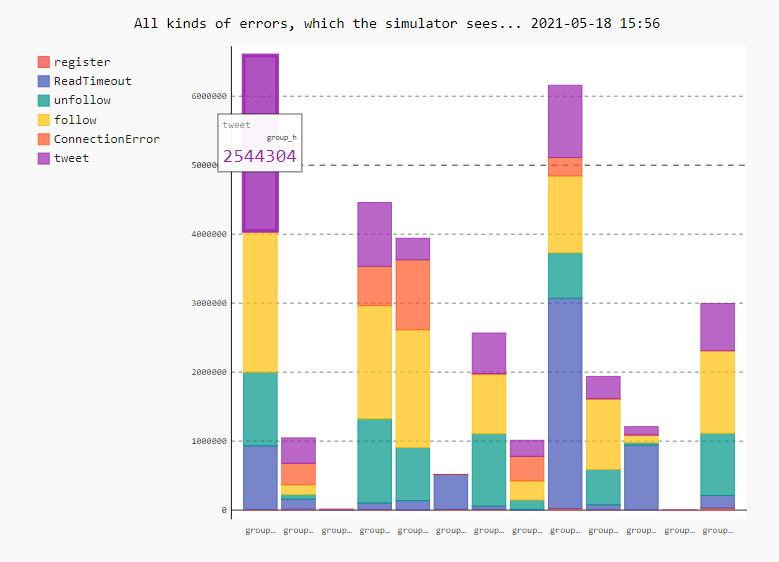
\includegraphics[width=1\textwidth]{images/simulatorerr.png}
\caption{\label{fig:sim} Simulator Errors}
\end{figure}

One reason to the large amount of http errors being created was, because of our pricing tier in Azure. We solved it by vertically scaling up our database tier allowing for more Database Transaction Units (DTU's). Another reason was responding with the wrong response code for quite some time. Another reason was that our API controller functioned very poorly in handling http requests. To solve this the http requests were divided up into simpler decoupled queries to avoid duplication of database calls, which ultimately optimized the performance.



\bibliographystyle{alpha}
\bibliography{sample}

\end{document}